\chapter{A Physical Perspective on The Rescue of Mutant CFTR}
\label{chap:perspective}
\chapquote {We have more problems than hands. }{- Eduardo Perozo (personal communication)}

\section{Introduction}

The preceding chapters have fit into some broad themes. Chapters \ref{chap:introduction} and \ref{chap:methods} outlined a philosophy of biological physics which we seek to use to understand Cystic Fibrosis. Meanwhile, chapters \ref{chap:cftr}-\ref{chap:opening} built up a molecular understanding of the root cause of Cystic Fibrosis, and demonstrating that small molecule drugs can rescue a diverse set of molecular phenotypes. In this chapter we will tie these results together. We will build a physical perspective on the rescue of mutant CFTR by potentiator drugs. A similar model could be built for corrector drugs, or even used to think about the modulation of any protein by small molecules.

We hope that this model will inform our current understanding of the action of CFTR modulators and also direct future efforts in treating the root cause of Cystic Fibrosis. We will outline specific studies motivated by this model in the next chapter.

We will begin with a brief overview of our results so far, analysing 4 rare CF-causing mutations which appear to respond to CFTR modulators even though they each have a unique molecular defect. We will then look at the molecular details of one of the best studied and most common disease causing Mutations G551D. 

We will show through simple unbiased MD, that this mutation causes a disruption to the binding of ATP, resulting in a gating defect. As with previous chapters, this gating defect appears unique, sharing little in common with the other gating defects we analysed previously. This array of different disease phenotypes leads us to propose a model based on the gating energy landscape, which accounts for the rescue of unique phenotypes by a class of drugs all acting with the same mechanism of action. 

We will demonstrate how to use this model to theratype a rare mutation at the molecular level. We will show how a poorly studied mutation, Q1291H appears to exhibit a similar molecular phenotype to G551D, leading us to expect that it will be amenable to potentiation by CFTR modulators, even though patients carrying this mutation are currently excluded from receiving modulator therapy. 

%Our simulations of G551D and Q1291H appear to show a similar molecular phenotyope, even though they occur on different parts of the protein. Q1291H is an extremely rare mutation, it has not been clinicarlly characteriesd and is not approved for treatment with modulators. So, by studying a common mutation, G551D and comparing it to Q1291H we give an example of theratyping of CF mutations from the molecular level.


\section{Summary Of Rare Mutations Studied so Far}

	\begin{center}
		\includegraphics[width=\textwidth]{figures/perspective/summary.pdf}
	\end{center}
\begingroup
\captionsetup{singlelinecheck = false, justification=raggedright}
\captionof {figure}[Summary of our Rare Mutation Studies] {\textbf{Summary of our Rare Mutation Studies}}{All of the mutations anlayised in this sthesis so far have been largely unique. They occur on different parts of the protein and cause misfunction through unique set of pathogenic interactions. Nonetheless, all of these mutations respond to potentiator class modulators. This situation demands that we tie together these reultes to explain how different pathogenicity can be treated by the same mecahnism of action. All of the mutations here have shown clinical benefit from the use of potenitaors, particularly in a triple combination therapy like Trikafta. } 
\endgroup

In chapter \ref{chap:I37R}, \ref{chap:R352Q}, \ref{chap:S945L} and \ref{chap:opening} we have analysed a disease causing mutation in detail in order to understand \textit{how} it caused CFTR to misfunction. What have found is a large diversity of molecular phenotypes which may cause disease. What is thus remarkable is that the \textit{in vitro} component of these papers all demonstrate that these mutations are responding to the same drugs, albeit with differing efficacies.

In chapters \ref{chap:I37R}-\ref{chap:opening} we demonstrated that a diverse set of molecular defects respond to CFTR modulators. Each of these defects displayed a response to CFTR potentiators. This means that even though the molecular origin of pathogenesis was unique, each defect could be treated by a common mechanism of action. This leads us to expect that the majority of disease causing missense mutations will be amenable to treatment via CFTR modulators, it is merely a problem of choosing the correct ones. 



\begin{itemize}
	\item Chapter \ref{chap:I37R} demonstrated that a novel form of pathogenesis arises from inter domain communications between the lasso motif and the R-domain.  This caused a class II gating defect. 
\item Chapter \ref{chap:R352Q} showed how a conductance class defect may arise from the deletion of a positive charge in the conduction pathway of the channel. The destruction of the salt bridge inside the channel may also affect the gating of the channel according to biochemical experiments \cite{}.
\item Chapter \ref{chap:S945L} showed how a stable network of hydrogen bonds allows the channel to fold correctly and aided in the gating cycle of the channel. 
\item Chapter \ref{chap:opening} demonstrated again that the deletion of a positive charge in the conduction pathway reduces anion conduction. However, this was in a completely different part of the channel compared to the R352Q study.
\end{itemize}


These molecular phenotypes are completely unique. They occur in completely different parts of the CFTR protein other on the CFTR protein. What is thus remarkable is that they all appear to respond to the same set of CFTR modulators in \textit{in vitro} experiments. There is no reason why we would expect CFTR proteins which differ from wild type only by missense mutations to not respond to these clearly very effective drugs.

\section{Analysing the Common G551D Gating Mutation}

In order to tie these results together, in this chapter I will propose a conceptual framework which explains how these drugs are able to treat such diverse molecular phenotypes. This model would appear to suggest that patients with rare missense mutations would be more likely to respond to respond to CFTR modulators. The implications of this model are also likely to inform the design of future generations of CFTR modulators. 

	\begin{center}
		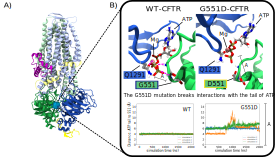
\includegraphics[width=\textwidth]{figures/perspective/G551D.pdf}
	\end{center}
\begingroup
\captionsetup{singlelinecheck = false, justification=raggedright}
\captionof {figure}[Summary of our Rare Mutation Studies] {\textbf{Summary of our Rare Mutation Studies}}{All of the mutations anlayised in this sthesis so far have been largely unique. They occur on different parts of the protein and cause misfunction through unique set of pathogenic interactions. Nonetheless, all of these mutations respond to potentiator class modulators. This situation demands that we tie together these reultes to explain how different pathogenicity can be treated by the same mecahnism of action.} 
\endgroup

\section{The Many Molecular Modes of CFTR Misfunction}
It is unlikely that the course classification of 6 classes conventionally used to understand CFTR mutants can be used to theratype patients, a granular, molecular understanding will be needed to choose which mutations can be rescued by modulators, and we outline some computational studies which might be performed to help understand how this would work.

\begin{landscape}
\begin{figure}
	\begin{center}
	%\includegraphics[angle=270,origin=c,width=0.38\textwidth]{figures/classes_mutations.pdf}\\
	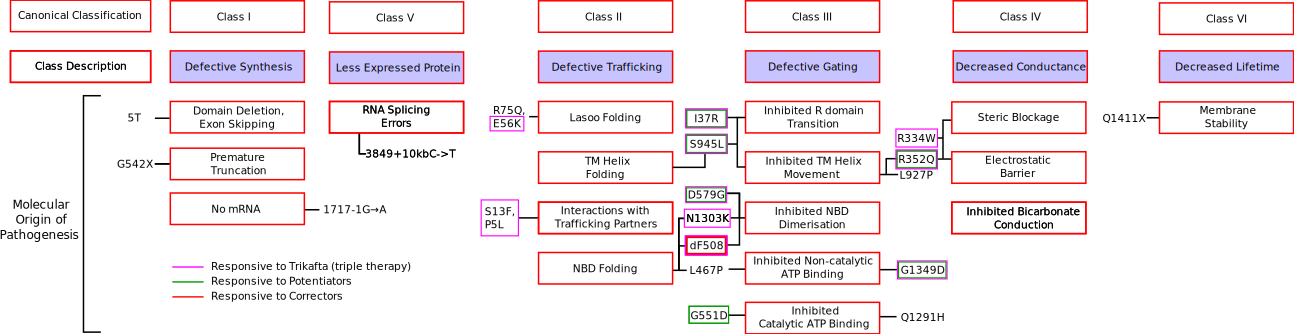
\includegraphics[width=1.5\textwidth]{figures/perspective/classes_mutations.pdf}\\
	\end{center}
	\captionsetup{singlelinecheck = false, justification=raggedright}
	\caption[Granular grouping of CF pathogenesis]{\textbf{Granular Grouping of Cystic Fibrosis Causing Mutations}{ Conventionally, CF genotypes are grouped into 7 classes of phenotype. These 7 classes, while useful are broad when one notes that the molecular details of misfunction can in fact be due to an array of factors. By realising that classification into a given class can be due to different factors we can gain a more complete  picture of the molecular cause of CF by delineating the molecular fingerprint of each mutation.}}

\end{figure}
\end{landscape}


\section{A Physics Motivated Approach to Precision Medicine in Cystic Fibrosis}

This model has important implications. We should be giving more patients modulators. Missense mutations likely represent a small perturbation to the folding and gating landscape of the WT channel and such . I assert that any heterogeneous response to modulators is not in fact to do with the mutation or the modulators them selves but likely involves other protein systems. Some of the uncertainty can be alleviated by the use of pre-clinical models which should be able to clear . Currently a range of missense mutations are recomended for treatment by trikafta but . Their current exclusion from accessing these therapies is errant. The above model suggests that when a patient carrying such a rare mutation does not respond to modulator therapy, it is unlikely that the lack of aresponse is due to the inability of these modulators to rescue the function of CFTR. From the perspective of protein physics, $\Delta$F508 is likely to perturb the protein much more than any missense mutation \cite{}. Rather, it is more likely that if a patient does not respond to modulators it is due to the broader heterogeneous response to modulators found in all patients. 

\section{The Poorly Studied Mutation Q1291H Produces a Similar Defect to G551D}

Through our molecular modelling we noticed another defect, Q1291H appears to produce a similar molecular defect to G551D even though it affects a different domain of CFTR. G551D is much more common than Q1291H and so patients carrying the former may access potentiators. However, Q1291H is extremely rare, so rare in fact it has not been well described clinically with only 30 alleles of this mutation recorded in CFTR2 \cite{cftr2}. A CF afflicted patient with this mutation presented to the Sydney children's hospital and is currently unable to access modulator therapy. Our modelling would lead us to believe that there is a high likelihood that cells carrying the Q1291H mutation would respond to potentiators or a combination therapy. 


As figure \ref{CF_life_expectancy} demonstrates back in chapter \ref{chap:cftr}, basic science discoveries concerning CF have had a direct effect on the life expectancy of patients. The work in this thesis is a small example of how abstract physical models, such as those outlined in \ref{chap:methods}, can be applied to help real patients in a community such as allowing patients in Sydney Children's hospital to access medications which could add decades to their life span. We are entering an exciting era of biophysical research where advances in theoretical methods, computing power and experimental techniques are beginning to drive advances in each other at a frenetic pace. An example can be seen in the development of Alphafold2. The maturation of cryoEM allowed the discovery of new protein folds which Alphafold2's machine learning algorithms could then learn from. Now that the algorithm had these folds in hand it could predict entire proteomes. This now means that structural biologists can use the predictions of alphafold to solve even more structures more quickly. Eventually, more and more of the experimental work currently involved in biology will move onto the silicon chip, while experimental techniques will advance in other areas. Similarly, the theoretical model argued for in this thesis will eventually allow for patient assessments to be made \textit{in silico}

The preceding chapters have given technical and molecular details about the cause of Cystic Fibrosis by rare genetic mutations, and further demonstrated that these mutations may be treated by existing small molecule drugs. The unique molecular fingerprint of each mutation indicates that in order to deliver better outcomes to patients a more personalised approach is necessary in the choice of medication. 


There is no reason to beleive that even in patients who do not show benefit from modulator therapy that the drugs are for some reason not reaching the CFTR protein. Infact, they seem to metabolise the drugs at teh same rate as patients who do. The success of preclinical models indicates that the problem is the cellular level and not at the level of organs or tissues. There is probably some genetic or cellular component that has not yet been identified which, once addressed, could bring the benefits of modulators to these patients.



In recent years there have been a slew of rare CF-causing genotypes discovered in populations with low rates of Cystic Fibrosis compared to Caucasians. These genotypes from Asia and the Middle East are often ultra-rare leading to poor outcomes for these patients \cite{}. 



	\begin{center}
	
\includegraphics[width=\textwidth]{figures/perspective/drug_landscape_1.pdf}\\
	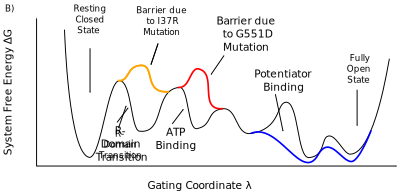
\includegraphics[width=\textwidth]{figures/perspective/drug_landscape_3.pdf}\\
	\end{center}
	\begingroup
	\captionsetup{singlelinecheck = false, justification=raggedright}
	\captionof{figure}[Conceptual Framework for the Pathogenesis of Mutations and The Action of Potentiators]{\textbf{Conceptual Framework for the Pathogenesis of Mutations and The Action of Potentiators}{ This model was produced to explain the apparent ability of CFTR modulators to treat rare mutations with a diverse set of phenotypes. A) The transition between the resting closed state and fully open state of CFTR can be visualised as a movement through an energy landscape. Along this transition various events must occur, such as the movement of the R-domain, ATP-binding and the rearrangements of the different domains of CFTR. Each of these events will have an energetic cost and payoff, giving rise to peaks and troughs in the free energy landscape of this transition. The relative heaths of peaks and troughs here are for illustrative purposes only, but quantitative techniques to calculate them will have important implications for the treatment of CF and drug discovery B) Gating class CF-causing mutations represent pathogenic barriers to this transition. They may effect different parts of the energy landscape. For example, we have shown that G551D causes a disruption to the binding of ATP, while in chapter \ref{chap:I37R}, we saw a gating defect arise in I37R-CFTR from the misregulation of the position of the R-domain. This demonstrates how pathogenesis can arise in many different ways in CFTR. Furthermore, accompanying \textit{in vitro} studies of these mutations demonstrated that these unique mutations each respond to potentiator class modulators. This indicates that the action of potentiators is \underline{somewhere else} in this free energy landscape, relative to the perturbation caused by mutation. By understanding \textit{where} mutations are causing gating inhibition and \textit{how} drugs are accounting for the deleterious energetics, we can begin to build a molecular basis for the choice of modulators, tailored to particular patients.}}
	\label{drug_action_model}

	\endgroup

The above model in figure \ref{drug_action_model} gives a rational, physical basis for the wide range of molecular phenotypes that CFTR modulators appear capable of treating. This same model would appear to argue that for most missense mutations we would expect them to respond to some sort of CFTR modulator. In short, the preceding chapters have shown that CFTR may misfunction by a wide range of defects. 

The ongoing discovery of rare mutations highlights the importance of this personalised approach to the treatment of CF. The process for developing potentiator class drugs was by studying the G551D mutation. Drugs that were found to restore function for this rare mutation are now widely used by sufferers of cystic fibrosis \cite{vangoor2009}. The study of rare mutations N1303K which currently do not respond to certain modulators may lead to the discovery of more effective compounds to treat cystic fibrosis such as. Thus, the approach to the treatment of Cystic Fibrosis is intersectional, as more rare mutations are discovered and treated the better the outcomes for all patients with Cystic Fibrosis will be. Each rare mutation sheds light on the function of CFTR and lets us understand and treat the root cause of the disease better.

\begin{figure}
	\begin{center}
		\includegraphics[width=\textwidth]{figures/perspective/Q1291.pdf}
	\end{center}
	\captionsetup{singlelinecheck = false, justification=raggedright}
	\caption[Molecular Basis of Q1291H-CFTR Pathogenesis]{\textbf{Molecular Basis of Q1291H-CFTR Pathogenesis.}{This mutation occurs on NBD2, in the vicinity of site 1, the catalytic ATP binding site. It appears as though this mutation also causes disruption to the binding of this ATP molecule, much like G551D. Q1291F is also included as it more reliably produces the molecular perturbation which we expect is characteristic of the Q1291H mutation. }}

\end{figure}

An analogous model could be drawn for the action of correctors. To do this we would need to clearly delineate the folding pathway of the CFTR protein and study how mutations cause aberrations in the folding landscape. Although work on this has begun \cite{krainer2018, kleizen2021, kleizen2020, fiedorczuk2022}, the folding pathway is much less straight forward to understand via simulations than the gating transition, so our proposed model will be detailed using the gating transition and potentiators.

The gating transition is simpler, as there are many easily measurable events which we can conceptualise, like ATP binding and pore formation. We will build our model with a focus on this aspect of protein function. Nonetheless, the concepts are transferable, to CFTR folding and as more corrector class drugs are developed and more mutant forms of CFTR are imaged we will gain more understanding f the folding pathway of this critical protein, so in time this model can be transferred to correctors as well. Additionally, as computer models improve we can simulate parts of this pathway as well. Computational capabilities are likely sufficiently advanced to simulate the full gating cycle of CFTR and so discover which parts of the landscape in figure \ref{drug_action_figure} are perturbed by mutations \cite{}. 

%These drugs are clinically efficacious \cite{VanGoor2014} on several mutants with some curious exceptions like N1303K. I suggest the following mechanism for their action. I suspect a similar analogy exists for the action of the correctors. WT-CFTR exhibits a natural landscape with kinetic barriers in the transition between the closed and open states. A gating class mutation to CFTR will introduce a kinetic barrier in the pathway of this conformational transition. What these drugs do is reduce a barrier in the existing conformational landscape of CFTR. This compensates for the barriers introduced by the mutation. j


\section{Summary}
In summary, the important findings from these 4 modelling studies demonstrate that many people with CF are likely to respond to modulator therapy, even though they excluded from these treatments by regulatory agencies. A biophysical methodology when considering the action of CFTR modulators leads us to expect that most patients carrying missense mutations will respond to modulator therapy.

By combining this molecular understanding with \textit{ex vivo} pre-clinical models it appears as as though CFTR modulators are capable of treating a diverse set of unique molecular defects. If the recomendations of this thesis are taken on board, eventually computational and molecular understanding of CFTR will sufficiently improved to make predictions about the repsonse of specific mutations to modulators.  

Currently, computational methods are not sufficiently developed in power or accuracy to theratype a mutation ab initio. Currently, we must rely heavily on the measurements of a patients' cells made \textit{in vitro}. However, as a more complete understanding of CF pathogenesis and patient genetics is built, we will be able to offload more and more of this clinical work onto computers.
